\begin{strip}
\centering
\begin{minipage}[t]{.325\linewidth}\centering
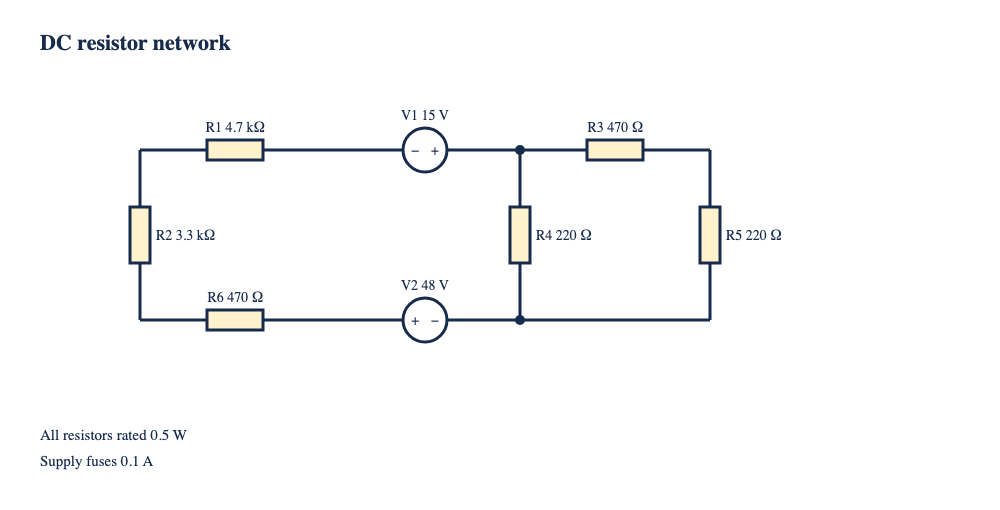
\includegraphics[width=\linewidth,trim=110 150 240 100,clip]{figures/teaser-dc_network-source.png}\\[-1pt]
{\footnotesize (a) Source drawing: \textbf{safe}}
\end{minipage}\hfill
\begin{minipage}[t]{.325\linewidth}\centering
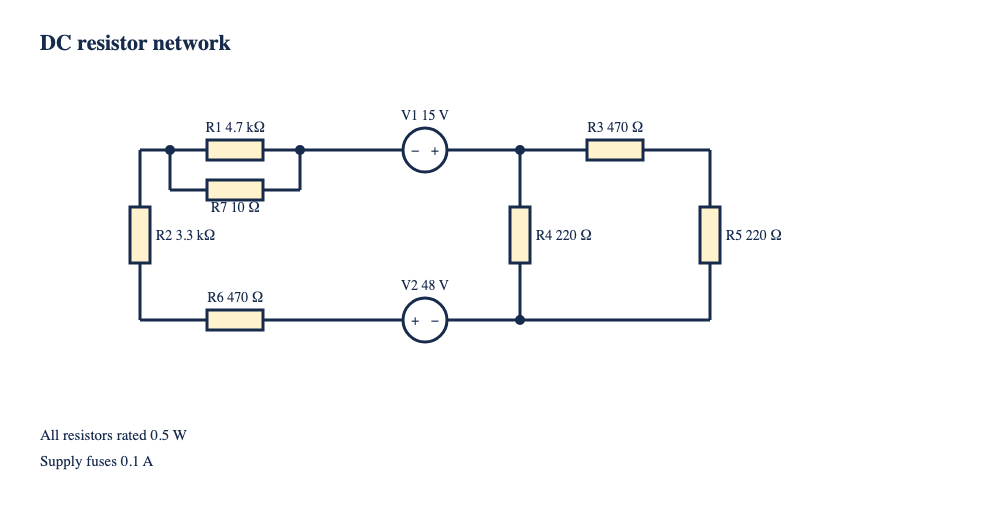
\includegraphics[width=\linewidth,trim=110 150 240 100,clip]{figures/teaser-dc_network-target.png}\\[-1pt]
{\footnotesize (b) ``Add R7 = 10\,$\Omega$ in parallel with R1.''}
\end{minipage}\hfill
\begin{minipage}[t]{.325\linewidth}\centering
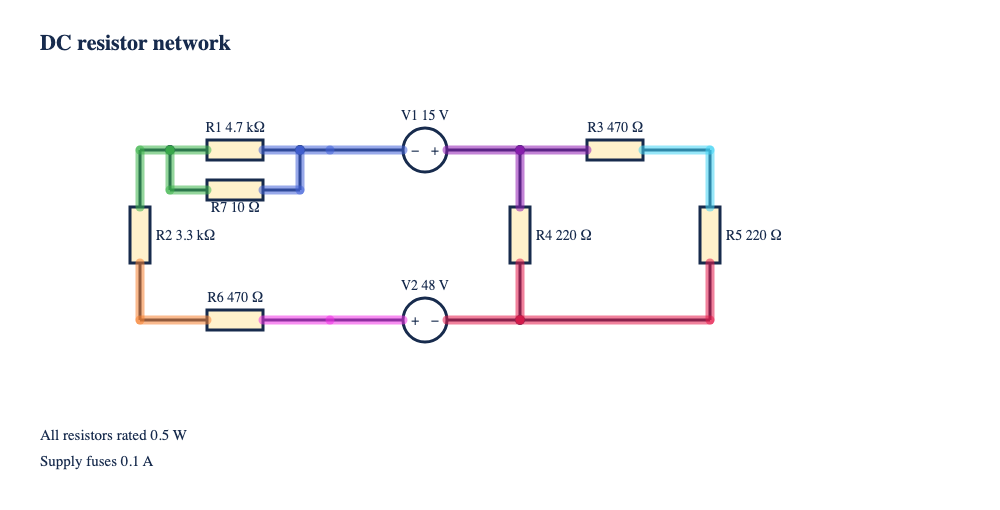
\includegraphics[width=\linewidth,trim=110 150 240 100,clip]{figures/teaser-dc_network-recovered.png}\\[-1pt]
{\footnotesize (c) Network recovered from (b): \textbf{unsafe}}
\end{minipage}
\captionsetup{hypcap=false}
\captionof{figure}{\textbf{Scoring an edit by re-solving the drawing.} A one-resistor edit to a two-source
network (a$\to$b) looks innocuous, but it overloads a component elsewhere in the circuit. \ours reads only
the visible SVG, rebuilding every electrical node from wire endpoints, T-junctions and junction dots (each
colour in (c) is one node), reading component values from their labels, and solving the network. Here the
edited drawing violates its own note: R2 now dissipates 0.84\,W against a 0.5\,W rating. The same procedure
scores any edited drawing, whoever or whatever produced it.}
\captionsetup{hypcap=true}
\label{fig:teaser}
\end{strip}
